%\begin{document}
%\section{Kissing ellipsoids}

In this section, we consider some circumstances in which there are two
principles and procedures for deriving estimates of a parameter vector $\vec{\beta}$
of a linear model,
each with its associated estimated variance-covariance matrix, e.g.,
$\widehat{\vec{\beta}}^A$ with covariance matrix $\widehat{\Var}(\hat{\vec{\beta}}^A)$,
and
$\widehat{\vec{\beta}}^B$ with covariance matrix $\widehat{\Var}(\hat{\vec{\beta}}^B)$.
We will take method A to be OLS estimation and consider several alternatives
for method B.  In $\beta$ space, the parameter estimates appear as points and their
corresponding confidence ellipsoids have the property that they will just ``kiss''
(or \emph{osculate}) along a path between the two estimates.
In the examples we consider, the alternative methods B represent a convex combination
of information from two sources and the path of osculation is interpretable in
terms of what method B aims to achieve.
The same geometric ideas can also be applied in data space, where we can consider
the data ellipsoids for two (or more) groups and find statistical interpretations of
their (pairwise) path of osculation.

These problems all have a similar and simple physical interpretation:  Imagine two stones dropped
into a pond at locations with coordinates $\vec{m}_1$ and $\vec{m}_2$.  The waves emanating from the centers
form concentric circles which osculate along the line from $\vec{m}_1$ to $\vec{m}_2$.
Now imagine a world with ellipse-generating stones, where instead of circles, the waves form concentric ellipses determined by
the shape matrices $\mat{A}_1$ and $\mat{A}_2$.
The \emph{locus of osculation} of these ellipses will be the set of points where the tangents
to the two ellipses are parallel (or equivalently, that their normals are parallel).  An
example is shown in \figref{fig:kiss-demo}, using $\vec{m}_1 = (-2, 2)$, $\vec{m}_2 = (2, 6)$, and
\begin{equation} \label{eq:kiss-demoA}
\mat{A}_1 = \left(
\begin{array}{cc}
 1.0 & 0.5 \\ 0.5 & 1.5
\end{array}
\right)
\comma\quad\quad
\mat{A}_2 =\left(
\begin{array}{cc}
 1.5 & -0.3 \\ -0.3 & 1.0
\end{array}
\right) \comma
\end{equation}
where we have found points of osculation by trial and error.  An exact analytic solution follows.

\begin{figure}[htb!]
  \centering
  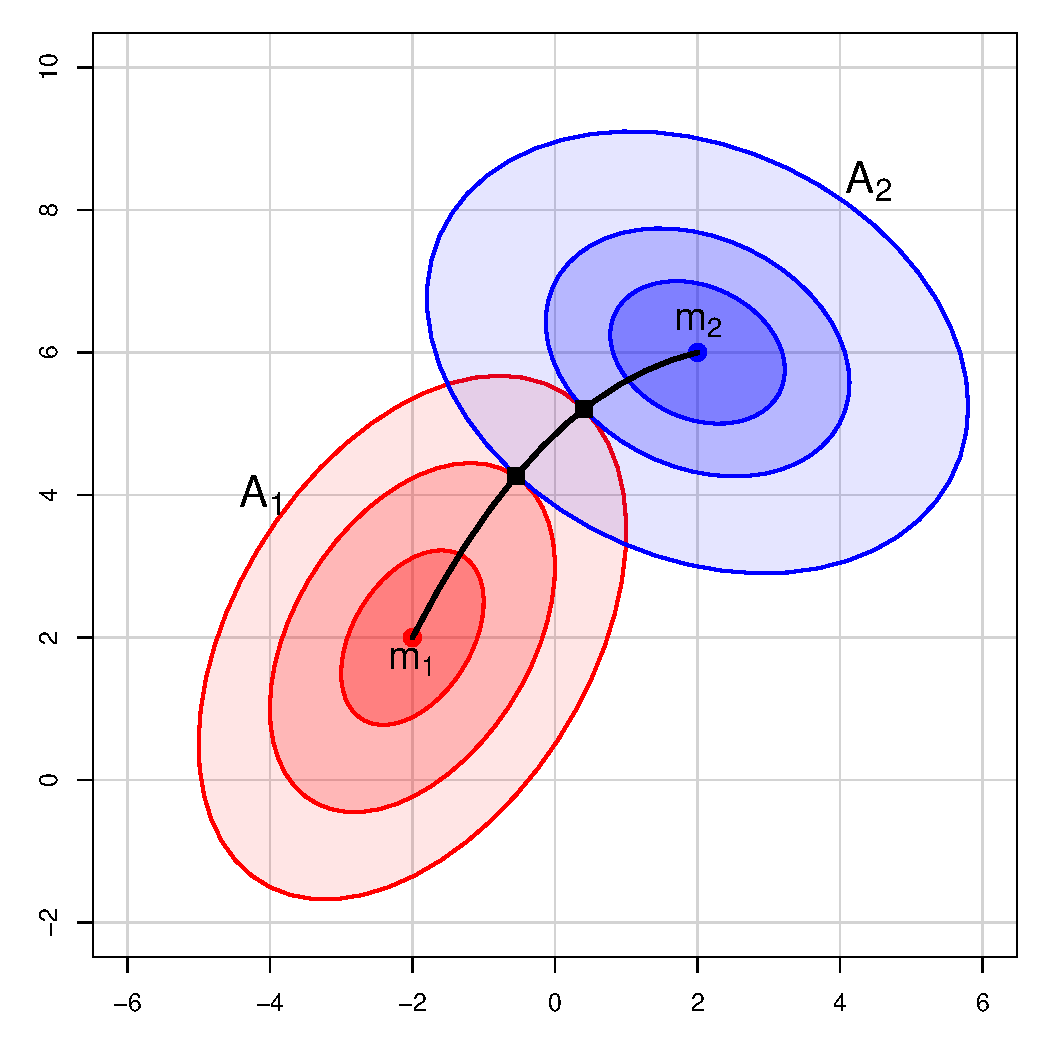
\includegraphics[width=.6\textwidth,clip]{fig/kiss-demo}
  \caption{Locus of osculation for two families of ellipsoidal level curves, with centers at $\vec{m}_1 = (-2, 2)$ and  $\vec{m}_2 = (2, 6)$,
  and shape matrices $\mat{A}_1$ and $\mat{A}_2$ given in \eqref{eq:kiss-demoA}.
  The left ellipsoids (red) have radii=1, 2, 3. The right ellipsoids
  have radii=1, 1.74, 3.1, where the last two values were chosen to make them kiss at the points marked with squares. The black curve is an
  approximation to the path of osculation, using a
  spline function connecting $\vec{m}_1$ to $\vec{m}_2$ via the marked points of osculation.}%
  \label{fig:kiss-demo}
\end{figure}

A general solution can be described as follows.  Let the ellipses be given by
\begin{eqnarray*}
f_1(\vec{x}) & = & \vec{m}_1 \oplus \sqrt{\mat{A}_1} = (\vec{x}-\vec{m}_1)\trans \mat{A}_1 (\vec{x}-\vec{m}_1) \\
f_2(\vec{x}) & = & \vec{m}_2 \oplus \sqrt{\mat{A}_2} = (\vec{x}-\vec{m}_2)\trans \mat{A}_2 (\vec{x}-\vec{m}_2) \comma \\
\end{eqnarray*}
and denote their gradient-vector functions as
\begin{equation}
\nabla f(x_1, x_2) = \left(\frac{\partial f}{\partial x_1}, \frac{\partial f}{\partial x_2} \right)
\end{equation}
so that
\begin{eqnarray*}
\nabla f_1(\vec{x}) & = & 2 \mat{A}_1 (\vec{x}-\vec{m}_1) \\
\nabla f_2(\vec{x}) & = & 2 \mat{A}_2 (\vec{x}-\vec{m}_2) \period \\
\end{eqnarray*}

Then, the points where $\nabla f_1$ and $\nabla f_2$ are parallel can be expressed in terms of the
condition that their vector cross product,
$\vec{u} \circledast \vec{v} = u_1 v_2 - u_2 v_1 = \vec{v}\trans \mat{C} \vec{u} = 0$, where \mat{C} is the skew-symmetric matrix
\begin{equation*}
\mat{C} = \left(
\begin{array}{cc}
 0 & 1 \\ -1 & 0
\end{array}
\right)
\end{equation*}
satisfying $\mat{C} = -\mat{C}\trans$.
Thus, the locus of osculation is the set $\mathcal{O}$, given by $\mathcal{O}  = \{\vec{x} \in \Real{2} \given \nabla f_1(\vec{x}) \circledast \nabla f_2(\vec{x}) = 0 \}$,
which implies
\begin{equation}
(\vec{x}-\vec{m}_2)\trans \, \mat{A}_2 \trans \: \mat{C} \: \mat{A}_1 \, (\vec{x}-\vec{m}_1) = 0  \period  \label{eq:locus}
\end{equation}
\eqref{eq:locus} is a biquadratic form in \vec{x}, with central matrix $\mat{A}_2 \trans \: \mat{C} \: \mat{A}_1$,
implying that $\mathcal{O}$ is a conic section in the general case. Note that when $\vec{x}=\vec{m}_1$ or $\vec{x}=\vec{m}_2$,
\eqref{eq:locus} is necessarily zero, so the locus of osculation always passes through  $\vec{m}_1$ and $\vec{m}_2$.

A visual demonstration of the theory above is
shown in \figref{fig:kiss-demo2} (left), which overlays the ellipses in \figref{fig:kiss-demo} with contour lines
(hyperbolae, here)
of
the vector cross-product function contained in \eqref{eq:locus}.
When the contours of $f_1$ and $f_2$ have the same shape ($\mat{A}_1 = c \mat{A}_2 $), as in the right panel of \figref{fig:kiss-demo2},
\eqref{eq:locus}
reduces to a line, in accord with the stones-in-pond interpretation.
The above can be readily extended to ellipsoids in higher dimension, where the development is more easily understood
in terms of normals to the surfaces.

\begin{comment}
\begin{figure}[htb!]
  \centering
  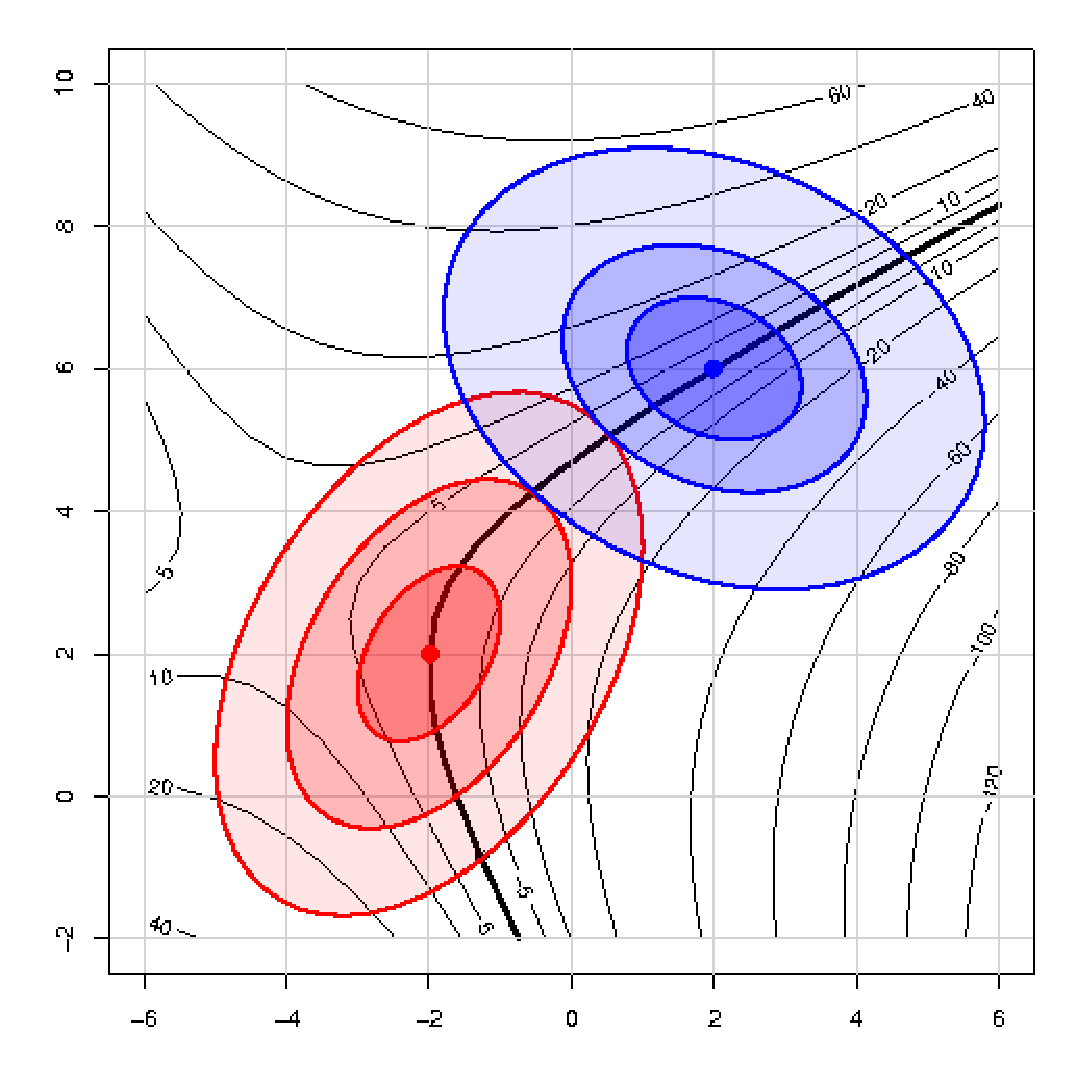
\includegraphics[width=.6\textwidth,clip]{fig/kiss-demo2}
  \caption{Locus of osculation for two families of ellipsoidal level curves, with parameters as in \figref{fig:kiss-demo} and \eqref{eq:kiss-demoA},
  showing contour lines of the vector cross-product function \eqref{eq:locus}.
  The thick black curve shows the complete locus of osculation for these two families of ellipses.}%
  \label{fig:kiss-demo2}
\end{figure}
\end{comment}

\begin{figure}[htb]
 \begin{minipage}[b]{.49\linewidth}
  \centering
  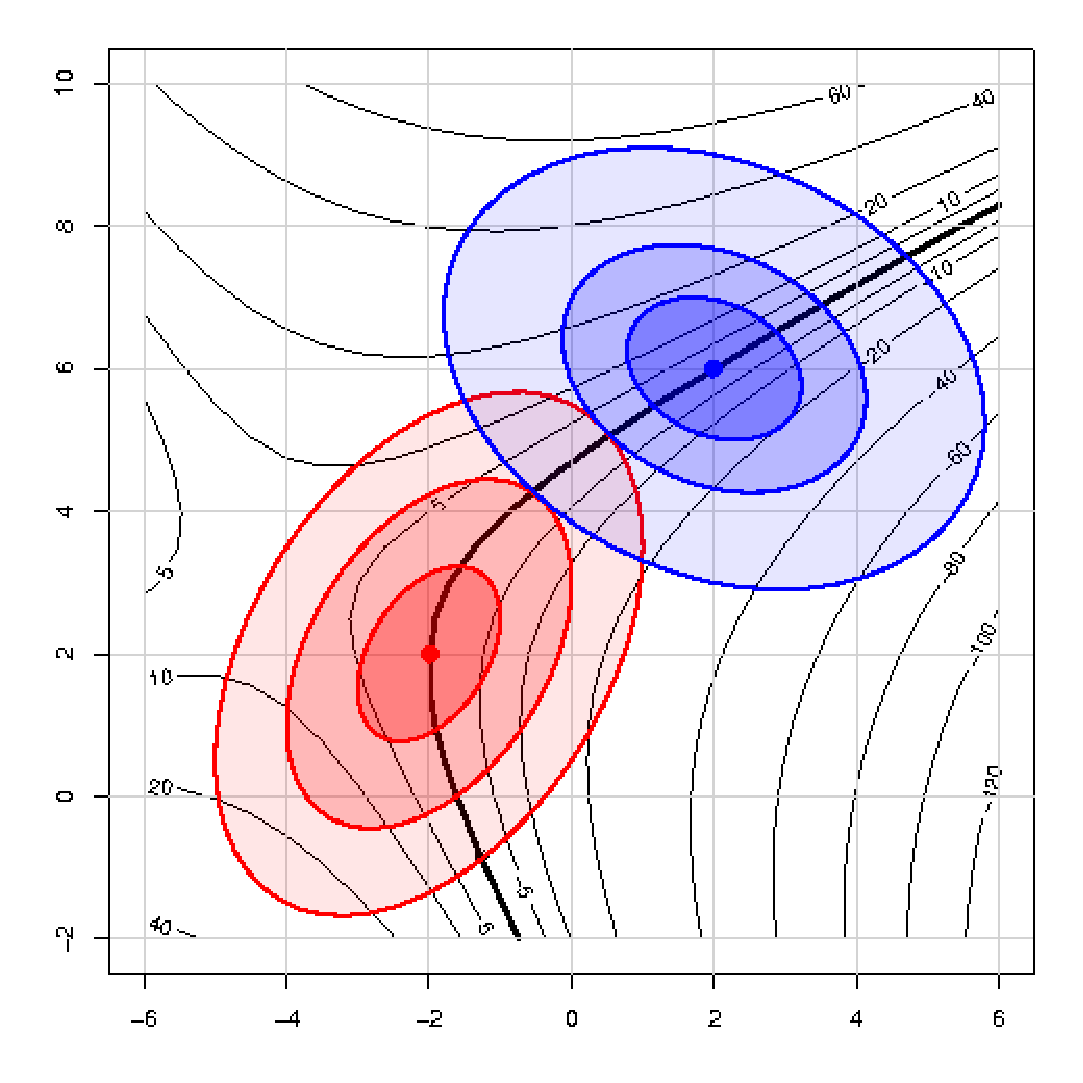
\includegraphics[width=1\linewidth]{fig/kiss-demo2a}
%  \caption{}%
%  \label{fig:}
 \end{minipage}%
 \hfill
 \begin{minipage}[b]{.49\linewidth}
  \centering
  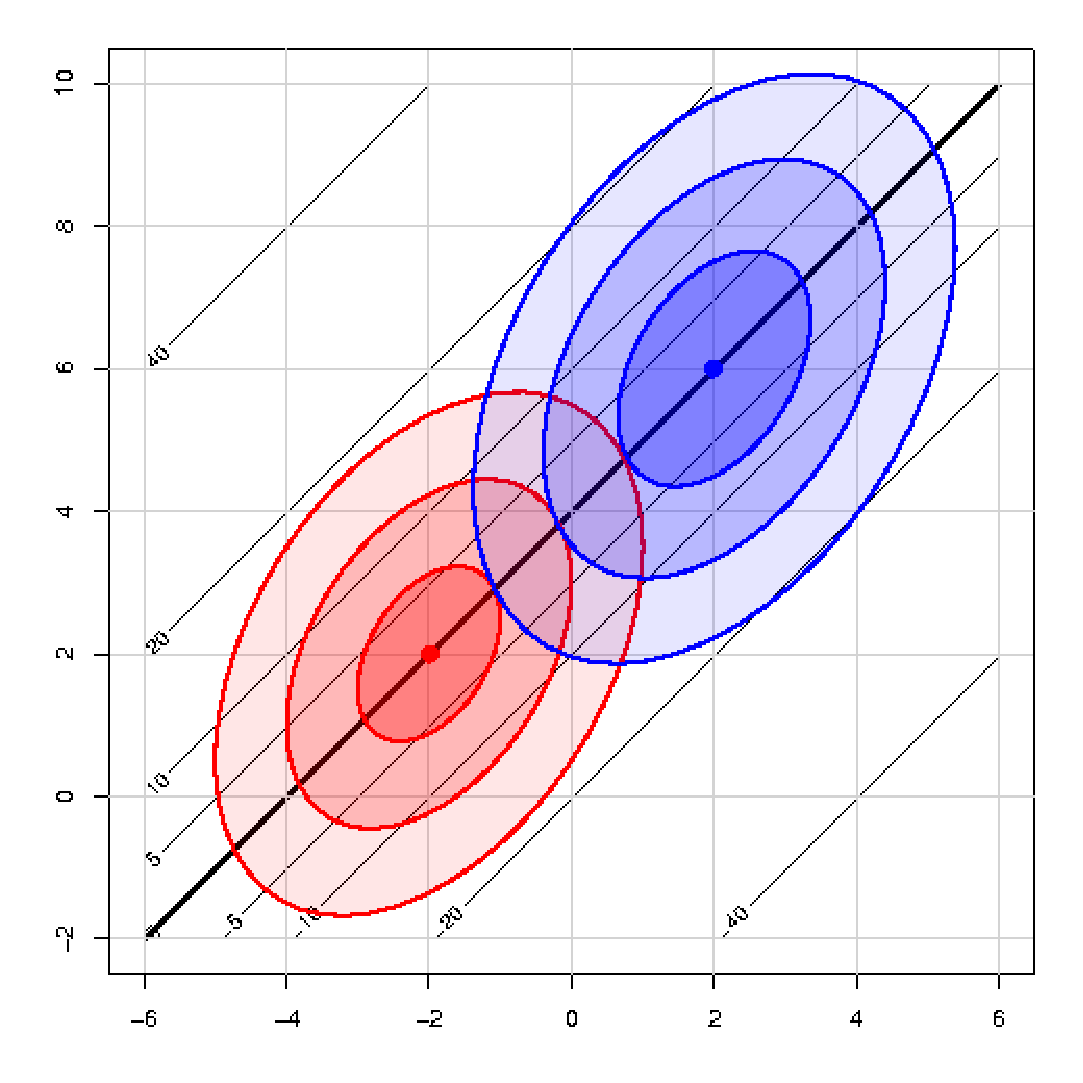
\includegraphics[width=1\linewidth]{fig/kiss-demo2b}
 \end{minipage}
  \caption{Locus of osculation for two families of ellipsoidal level curves, showing contour lines of the vector cross-product function \eqref{eq:locus}.
  The thick black curve shows the complete locus of osculation for these two families of ellipses, where the cross-product function equals 0.
Left:~with parameters as in \figref{fig:kiss-demo} and \eqref{eq:kiss-demoA}. Right:~with the same shape matrix $\mat{A}_1$ for both
ellipsoids.}
  \label{fig:kiss-demo2}
\end{figure}
%\end{document}
